% Festlegung des Allgemeinen Dokumentenformats
\documentclass[a4paper,12pt,headsepline]{scrartcl}

% Umlaute unter UTF8 nutzen
\usepackage[utf8]{inputenc}

% Variablen
%Variablen welche innerhalb der gesamten Arbeit zur Verfügung stehen sollen
\newcommand{\titleDocument}{Regenvorhersage mit Neuronalen Netzen und die Visualisierung dieser in einer App}
\newcommand{\subjectDocument}{MSI AS - Master Informatik, Autonome Systeme}


% weitere Pakete
% Grafiken aus PNG Dateien einbinden
%\usepackage{graphicx}
\usepackage[export]{adjustbox}
\usepackage{float}
\usepackage{subfig}
% aus SVG
\usepackage{svg}

% Deutsche Sonderzeichen und Silbentrennung nutzen
\usepackage[ngerman]{babel}

% Eurozeichen einbinden
\usepackage[right]{eurosym}

% Zeichenencoding
\usepackage[T1]{fontenc}

\usepackage{lmodern}

% floatende Bilder ermöglichen
%\usepackage{floatflt}

% mehrseitige Tabellen ermöglichen
\usepackage{longtable}

% Unterstützung für Schriftarten
%\newcommand{\changefont}[3]{ 
%\fontfamily{#1} \fontseries{#2} \fontshape{#3} \selectfont}

% Packet für Seitenrandabständex und Einstellung für Seitenränder
\usepackage{geometry}
\geometry{left=3cm, right=3cm, top=2.5cm, bottom=2cm}

% Paket für Boxen im Text
\usepackage{fancybox}

% bricht lange URLs "schön" um
\usepackage[hyphens,obeyspaces,spaces]{url}

% Paket für Textfarben
\usepackage{color}

% Mathematische Symbole importieren
\usepackage{amssymb}

% auf jeder Seite eine Überschrift (alt, zentriert)
%\pagestyle{headings}

% erzeugt Inhaltsverzeichnis mit Querverweisen zu den Abschnitten (PDF Version)
\usepackage[bookmarksnumbered,pdftitle={\titleDocument},hyperfootnotes=false]{hyperref}
%\hypersetup{colorlinks, citecolor=red, linkcolor=blue, urlcolor=black}
%\hypersetup{colorlinks, citecolor=black, linkcolor= black, urlcolor=black}

% neue Kopfzeilen mit fancypaket
\usepackage{fancyhdr} %Paket laden
\pagestyle{fancy} %eigener Seitenstil
\fancyhf{} %alle Kopf- und Fußzeilenfelder bereinigen
\fancyhead[L]{\nouppercase{\leftmark}} %Kopfzeile links
\fancyhead[C]{} %zentrierte Kopfzeile
\fancyhead[R]{\thepage} %Kopfzeile rechts
\renewcommand{\headrulewidth}{0.2pt} %obere Trennlinie
%\fancyfoot[C]{\thepage} %Seitennummer
%\renewcommand{\footrulewidth}{0.4pt} %untere Trennlinie

% für Tabellen
\usepackage{array}

% Runde Klammern für Zitate
%\usepackage[numbers,round]{natbib}

% Festlegung Art der Zitierung - Havardmethode: Abkuerzung Autor + Jahr
\bibliographystyle{alphadin}

% Schaltet den zusätzlichen Zwischenraum ab, den LaTeX normalerweise nach einem Satzzeichen einfügt.
%\frenchspacing

% Paket für Zeilenabstand
\usepackage{setspace}

% für Bildbezeichner
\usepackage{capt-of}

% für Stichwortverzeichnis
\usepackage{makeidx}

% für Listings
\usepackage{listings}
\lstset{numbers=left, numberstyle=\tiny, numbersep=5pt, keywordstyle=\color{black}\bfseries, stringstyle=\ttfamily,showstringspaces=false,basicstyle=\footnotesize,captionpos=b}
\lstset{language=java}

% Indexerstellung
\makeindex


% Abkürzungsverzeichnis TeTEX Version
% \usepackage[german]{nomencl}
% \makenomenclature
% %\makeglossary
% \renewcommand{\nomname}{Abkürzungsverzeichnis}
% \AtBeginDocument{\setlength{\nomlabelwidth}{.25\columnwidth}}
% \renewcommand{\nomlabel}[1]{#1 \dotfill}
% \setlength{\nomitemsep}{-\parsep}

% Optional: Einzelne Zeilen am Anfang einer Seite unterdrücken (Schusterjungen)
% \clubpenalty = 10000
% Optional: Einzelne Zeilen am Ende einer Seite unterdrücken (Hurenkinder)
% \widowpenalty = 10000
% \displaywidowpenalty = 10000

\begin{document}
% hier werden die Trennvorschläge inkludiert
%hier müssen alle Wörter rein, welche Latex von sich auch nicht korrekt trennt bzw. bei denen man die genaue Trennung vorgeben möchte
\hyphenation{
Film-pro-du-zen-ten
Lux-em-burg
Soft-ware-bau-steins
zeit-in-ten-siv
}


% Schriftart Helvetica verwenden
%\usepackage{helvet}
%\renewcommand\familydefault{\sfdefault}

% Titelseite %
\thispagestyle{empty}


\begin{figure}[t]
 \centering
 
\includegraphics[width=0.2\textwidth]{abb/regenschirm}
\end{figure}


\begin{verbatim}


\end{verbatim}

\begin{center}
\Large{HTWG Konstanz}\\
\end{center}

\begin{center}
\Large{Fakultät für Informatik}
\end{center}
\begin{verbatim}




\end{verbatim}
\begin{center}
\textbf{\LARGE{DeepRain}} \\
\vspace{1cm}
\doublespacing
\textbf{\LARGE{\titleDocument}}\\
\singlespacing
\begin{verbatim}

\end{verbatim}
\textbf{{~\subjectDocument}}
\end{center}
\begin{verbatim}

\end{verbatim}
\begin{center}

\end{center}
\begin{verbatim}


\end{verbatim}
\begin{flushleft}
\begin{tabular}{llll}
\textbf{Autoren:} & & Simon Christofzik& \\
& & Paul Sutter& \\
& & Till Reitlinger \\
& & \\
\textbf{Version vom:} & & \today &\\
& & \\
\textbf{Betreuer:} & & Prof. Dr. Oliver Dürr &\\
\end{tabular}
\end{flushleft}


% römische Numerierung
\pagenumbering{roman}

% 1.5 facher Zeilenabstand
\onehalfspacing

\newpage

% einfacher Zeilenabstand
\singlespacing

\newpage
% Seitenzählung bei Inhaltsverzeichnis beginnen
\setcounter{page}{1}

% Inhaltsverzeichnis anzeigen
\thispagestyle{empty}
\tableofcontents


% Verion 2: Abbildungsverzeichnis OHNE führende Nummberierung endgueltig anzeigen
%\begingroup
%\renewcommand\numberline[1]{}
%\listofs
%\endgroup


% das Tabellenverzeichnis
%\newpage
% Tabellenverzeichnis soll im Inhaltsverzeichnis auftauchen
%\addcontentsline{toc}{section}{Tabellenverzeichnis}
% \fancyhead[L]{Abbildungsverzeichnis / Abkürzungsverzeichnis} %Kopfzeile links
% Tabellenverzeichnis endgültig anzeigen
%\listoftables

%% WORKAROUND für Listings
%\makeatletter% --> De-TeX-FAQ
%\renewcommand*{\lstlistoflistings}{%
%  \begingroup
%    \if@twocolumn
%      \@restonecoltrue\onecolumn
%    \else
%      \@restonecolfalse
%    \fi
%    \lol@heading
%    \setlength{\parskip}{\z@}%
%    \setlength{\parindent}{\z@}%
%    \setlength{\parfillskip}{\z@ \@plus 1fil}%
%    \@starttoc{lol}%
%    \if@restonecol\twocolumn\fi
%  \endgroup
%}
%\makeatother% --> \makeatletter
% das Listingverzeichnis
%\newpage
% Listingverzeichnis soll im Inhaltsverzeichnis auftauchen
%\addcontentsline{toc}{section}{Listingverzeichnis}
%\fancyhead[L]{Listingverzeichnis} %Kopfzeile links
%\renewcommand{\lstlistlistingname}{Listingverzeichnis}
%\lstlistoflistings
%%%%

%%%%%%% EINLEITUNG %%%%%%%%%%%%
\newpage
\fancyhead[L]{\nouppercase{\leftmark}} %Kopfzeile links

% 1,5 facher Zeilenabstand
\onehalfspacing

% arabische Seitennummerierung ab hier
\pagenumbering{arabic}

\section{Einleitung}
In Quasi allen Zweigen der Wirtschaft spielt das Wetter eine Rolle welche das Handeln und den wirtschaftlichen Erfolg beeinflusst.
Angefangen beim Bäcker, dessen Personalplanung und Brötchenmenge vom Grillwetter abhängt, 
bis zur Landwirtschaft, in welcher der Anbau und Erntezeitpunkt auf Grundlage der Wettervorhersagen getroffen werden muss. 
Außerdem finden Wettervorhersagen selbstverständlich auch im privaten Sektor große Anwendung und werden von den meisten Menschen täglich verwendet. 
Während die Vorhersage von Temperaturen und Sonnenstunden mit Physikalischen Modellen inzwischen sehr zuverlässig funktionieren, 
sind Regenvorhersagen verhältnismäßig schwer zu machen. Nicht umsonst werden Regenvorhersagen in den meisten Fällen nur mit Wahrscheinlichkeiten angegeben. 
Das liegt vor allem an der immens großen Anzahl von Faktoren welche den Regen beeinflussen. 
Laut dem Deutschen Wetterdienst sind aktuell nur 80\% der Regenvorhersagen korrekt, bei den Temperaturen hingegen sind es über 90\% \cite{SpiegelWetter}. 
Der Rechenaufwand für Wettervorhersagen ist Enorm aber aufgrund der beschriebenen Relevanz werden die nötigen Ressourcen eingesetzt um ausreichend gute Wettervorhersagen zu ermöglichen.
In Deutschland gibt es mit dem Deutschen Wetterdienst eine Behörde die meteorologischen Dienstleistungen für die Allgemeinheit erbringt.
Diese werden im Folgenden auch in Anspruch genommen.      
\noindent Neuronale Netzte können dabei helfen in diesen komplexen und teilweise chaotisch wirkenden Vorgängen Muster zu erkennen und so Regenvorhersagen zu berechnen. 


\section{deep\_rain\_app}
In diesem Ordner befindet sich der gesamte Code, der für jegliche Funktionalitäten der App benötigt wird. 
Dazu gehört der Eigentliche App Code (deep\_rain), die Cloudfunction, welche für die Pushbenachrichtigung benötigt wird (FlutterCloudFunction),
sowie der Serversimulator (deeprainFireBase). 

\subsection{deep\_rain}
Die relevanten Ordner sind lib und assets. 
\subsubsection{assets}
Hier befinden sich alle in der App benötigten Bilder, sowie andere statische Daten. 
Dazu gehören zum Beispiel die Listen mit hilfe welcher der Pixel in den Vorhersage PNGs berechnet werden kann (data). 

\subsubsection{lib}
In diesem Ordner befindet sich der komplette, selbst geschriebene, Flutter Code. 
\subsubsection*{DataObjects}
In diesem Ordner befinden sich die Klasse, welche die Vorhersage PNGs speichert (DataHolder), sowie
die Klasse die das Objekt beschreibt, welches in der Liste angezeigt wird (ForecastListItem).
\subsubsection*{global}
In diesem Ordner befinden sich zwei Datenklassen welche von der gesamten App verwendet werden. 
In der Datei GlobalValues befinden sich alle global gespeicherten Variablen.
In der Datei UIText befinden sich alle angezeigten Texte in verschiedenen Sprachen. 
\subsubsection*{screens}
Es gibt für jeden Screen eine Datei in dem Ordner screens. Diese werden über die Datei main.dart verwaltet. 
\subsubsection*{Services}
Database.dart kümmert sich um die Kommunktion mit der Datenbank und ist die einzige Klasse, welche direkt mit der Datenbank 
kommuniziert. Alle Datenbank aktionen laufen über diese Klasse. 
FindPixel.dart stellt eine Funktion zur Verfügung, mit welcher es möglich ist, den eigenen Pixel im Vorhersage PNG zu finden. 
ProvideForecastData stellt die aktuellen ForecastListItems für die Forecast List zur verfügung. 
In PushNotification.dart wird festgelegt, wie sich die App bei dem öffnen und erhalten einer Pushbenachrichtigung verhalten soll. 
\subsubsection*{Widgets}
Die beiden .dart Dateien in diesem Ordner legen fest, wie die ForecastListe aussehen soll. forecast\_list\_widget stellt 
dabei die gesamte Liste dar, forecast\_tile nur eine Zeile aus der Liste. 

\subsection{deepRainFireBase}
Database.py simuliert den Server, wenn dieser nicht aktiv ist. 
Es werden Regenvorhersagen in die Datenbank geladen und Push Benachrichtigungen getriggert.
Viele Teile dieser Klasse sind später auch Teil der verwendeten Pipeline geworden. 
Diese Klasse ist nur ein Werkzeug, um die weiterentwicklung der App zu vereinfachen. 

\subsection{FlutterCloudFunction}
In dem Ordner functions, befindet sich in der Datei index.js die eigentliche CloudFunktion.
Die Funktionsweise dieser Funktion ist in der Hauptdokumentation ausgeführt. 
Um die änderungen an der CloudFunktion zu veröffentlichen und anzuwenden, muss diese zuerst über die Konsole 
deployed werden. 


\newpage

% In dieser Datei ist viel Beispielcode für alle möglichen Arten von Formattierungen usw.
%% einzelne Kapitel werden hier eingebunden
\section{Einleitung}\label{einleitung}

Hier steht die Einleitung der Arbeit... Lorem ipsum dolor sit amet, consetetur sadipscing elitr, sed diam nonumy eirmod tempor invidunt ut labore et dolore magna aliquyam erat, sed diam voluptua. At vero eos et accusam et justo duo dolores et ea rebum. Stet clita kasd gubergren, no sea takimata sanctus est Lorem ipsum dolor sit amet. Lorem ipsum dolor sit amet, consetetur sadipscing elitr, sed diam nonumy eirmod tempor invidunt ut labore et dolore magna aliquyam erat, sed diam voluptua. At vero eos et accusam et justo duo dolores et ea rebum. Stet clita kasd gubergren, no sea takimata sanctus est Lorem ipsum dolor sit amet.

\newpage

\section{Hauptabschnitt}\label{hauptabschnitt}

Text des ersten Abschnitts... Lorem ipsum dolor sit amet, consetetur sadipscing elitr, sed diam nonumy eirmod tempor invidunt ut labore et dolore magna aliquyam erat, sed diam voluptua. At vero eos et accusam et justo duo dolores et ea rebum. Stet clita kasd gubergren, no sea takimata sanctus est Lorem ipsum dolor sit amet. Lorem ipsum dolor sit amet, consetetur sadipscing elitr, sed diam nonumy eirmod tempor invidunt ut labore et dolore magna aliquyam erat, sed diam voluptua. At vero eos et accusam et justo duo dolores et ea rebum. Stet clita kasd gubergren, no sea takimata sanctus est Lorem ipsum dolor sit amet.

\subsection{Unterabschnitt 1}\label{unterabschnitt_1}

Erstes Unterabschnitt

\subsection{Unterabschnitt 2}\label{unterabschnitt_2}

Zweites Unterabschnitt

\subsection{Unterabschnitt 3}\label{unterabschnitt_3}

Drittes Unterabschnitt

\newpage

\section{Weiterer Hauptabschnitt}\label{hauptabschnitt_2}

Text des zweiten Abschnitts... Lorem ipsum dolor sit amet, consetetur sadipscing elitr, sed diam nonumy eirmod tempor invidunt ut labore et dolore magna aliquyam erat, sed diam voluptua. At vero eos et accusam et justo duo dolores et ea rebum. Stet clita kasd gubergren, no sea takimata sanctus est Lorem ipsum dolor sit amet. Lorem ipsum dolor sit amet, consetetur sadipscing elitr, sed diam nonumy eirmod tempor invidunt ut labore et dolore magna aliquyam erat, sed diam voluptua. At vero eos et accusam et justo duo dolores et ea rebum. Stet clita kasd gubergren, no sea takimata sanctus est Lorem ipsum dolor sit amet.

\newpage

% hier können weitere Kapitel angelegt und eingetragen werden
% ....

\section{Ausblick}\label{ausblick}

Text des Ausblicks - sofern dies in der Arbeit gewünscht ist... Lorem ipsum dolor sit amet, consetetur sadipscing elitr, sed diam nonumy eirmod tempor invidunt ut labore et dolore magna aliquyam erat, sed diam voluptua. At vero eos et accusam et justo duo dolores et ea rebum. Stet clita kasd gubergren, no sea takimata sanctus est Lorem ipsum dolor sit amet. Lorem ipsum dolor sit amet, consetetur sadipscing elitr, sed diam nonumy eirmod tempor invidunt ut labore et dolore magna aliquyam erat, sed diam voluptua. At vero eos et accusam et justo duo dolores et ea rebum. Stet clita kasd gubergren, no sea takimata sanctus est Lorem ipsum dolor sit amet.

\newpage

\section{Fazit}\label{fazit}

Text des Fazits... Lorem ipsum dolor sit amet, consetetur sadipscing elitr, sed diam nonumy eirmod tempor invidunt ut labore et dolore magna aliquyam erat, sed diam voluptua. At vero eos et accusam et justo duo dolores et ea rebum. Stet clita kasd gubergren, no sea takimata sanctus est Lorem ipsum dolor sit amet. Lorem ipsum dolor sit amet, consetetur sadipscing elitr, sed diam nonumy eirmod tempor invidunt ut labore et dolore magna aliquyam erat, sed diam voluptua. At vero eos et accusam et justo duo dolores et ea rebum. Stet clita kasd gubergren, no sea takimata sanctus est Lorem ipsum dolor sit amet.


% Beispiel für Bild mit Fußnote
\begin{figure}[htb]
 \centering
 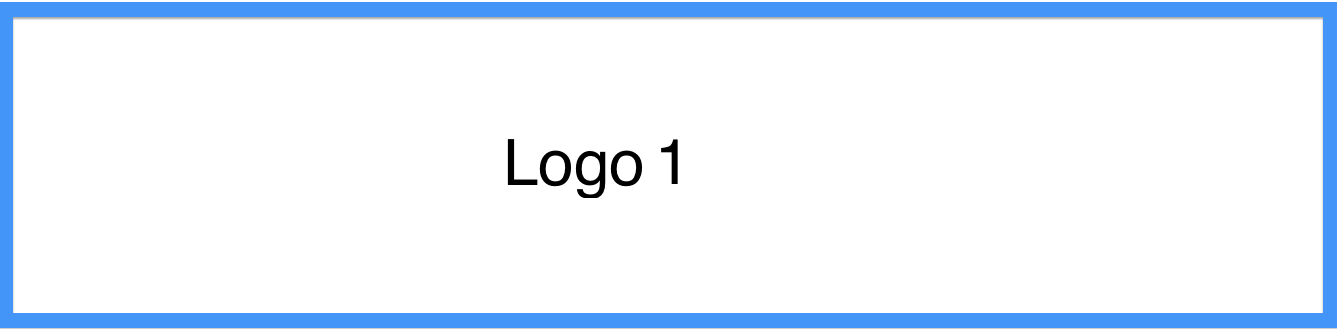
\includegraphics[width=0.4\textwidth,angle=45]{abb/logo1}
 \caption[Beispiel einer Bildbeschreibung]{Beispiel einer Bildbeschreibung\footnotemark}
\label{fig:beispiel1}
\end{figure}
\footnotetext{Bildquelle: Beispiel einer Bildquelle}

% Beispiel für Bildintegration
\begin{figure}[htb]
 \centering
 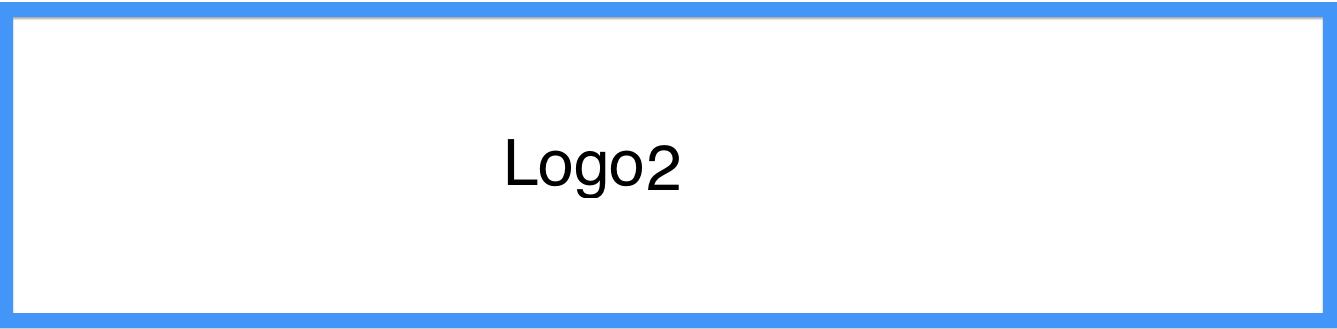
\includegraphics[width=0.3\textwidth,angle=0]{abb/logo2}
 \caption[Beschreibung]{Beschreibung}
\label{fig:Beschreibung}
\end{figure}

% Beispiel: Referenz auf Abbildung
Abbildung~\ref{fig:Beschreibung} [S.\pageref{fig:Beschreibung}]

% Beispiel: Tabelle 
\begin{center}
  \begin{tabular}{ | l | c | }
    \hline
    Überschrift 1 & Überschrift 2 \\ \hline \hline
    Info 1 & Info 2 \\ \hline
    Info 3 & Info 4 \\ \hline
    \hline
    \multicolumn{2}{|c|}{Info in einer Zelle} \\
    \hline
  \end{tabular}
\end{center}


% Beispiel für Quellcode Listings
\lstset{language=xml}
\begin{lstlisting}[frame=htrbl, caption={Die Datei {\normalfont \ttfamily  data-config.xml} dient als Beispiel für XML Quellcode}, label={lst:dataconfigxml}]
<dataConfig>
  <dataSource type="JdbcDataSource" 
              driver="com.mysql.jdbc.Driver"
              url="jdbc:mysql://localhost/bms_db"
              user="root" 
              password=""/>
  <document>
    <entity name="id"
        query="select id, htmlBody, sentDate, sentFrom, subject, textBody
        from mail">
    <field column="id" name="id"/>
    <field column="htmlBody" name="text"/>
    <field column="sentDate" name="sentDate"/>
    <field column="sentFrom" name="sentFrom"/>
    <field column="subject"  name="subject"/>
    <field column="textBody" name="text"/>
    </entity>
  </document>
</dataConfig>
\end{lstlisting}

\lstset{language=java}
\begin{lstlisting}[frame=htrbl, caption={Das Listing zeigt Java Quellcode}, label={lst:result2}]
/* generate TagCloud */
Cloud cloud = new Cloud();
cloud.setMaxWeight(_maxSizeOfText);
cloud.setMinWeight(_minSizeOfText);
cloud.setTagCase(Case.LOWER);
	    
/* evaluate context and find additional stopwords */
String query = getContextQuery(_context);
List<String> contextStoplist = new ArrayList<String>();
contextStoplist = getStopwordsFromDB(query);
	    
/* append context stoplist */
while(contextStoplist != null && !contextStoplist.isEmpty())
  _stoplist.add(contextStoplist.remove(0));
	    
/* add cloud filters */
if (_stoplist != null) {
  DictionaryFilter df = new DictionaryFilter(_stoplist);
  cloud.addInputFilter(df);
}
/* remove empty tags */
NonNullFilter<Tag> nnf = new NonNullFilter<Tag>();
cloud.addInputFilter(nnf);

/* set minimum tag length */
MinLengthFilter mlf = new MinLengthFilter(_minTagLength);
cloud.addInputFilter(mlf);

/* add taglist to tagcloud */
cloud.addText(_taglist);

/* set number of shown tags */	    
cloud.setMaxTagsToDisplay(_tagsToDisplay);
\end{lstlisting}


% Beispiel für Formeln
Die Zuordnung aller möglichen Werte, welche eine Zufallsvariable annehmen kann nennt man \emph{Verteilungsfunktion} von $X$.

\begin{quotation}
Die Funktion F: $\mathbb{R} \rightarrow$ [0,1] mit $F(t) = P (X \le t)$ heißt Verteilungsfunktion von $X$.\footnote{Mustermann, vgl.~\cite{mm2009}~[S.55]}
\end{quotation}

\begin{quotation}
Für eine stetige Zufallsvariable $X: \Omega \rightarrow \mathbb{R}$ heißt eine integrierbare, nichtnegative reelle Funktion $w: \mathbb{R} \rightarrow \mathbb{R}$ mit $F(x) = P(X \le x) = \int_{-\infty}^{x} w(t)dt$ die \emph{Dichte} oder \emph{Wahrscheinlichkeitsdichte} der Zufallsvariablen $X$.\footnote{Mustermann, vgl.~\cite{mf2005}~[S.56]}
\end{quotation}


% einfacher Zeilenabstand
\singlespacing
% Literaturliste soll im Inhaltsverzeichnis auftauchen
\newpage
\addcontentsline{toc}{section}{Literaturverzeichnis}
% Literaturverzeichnis anzeigen
\renewcommand\refname{Literaturverzeichnis}
\bibliography{Hauptdatei}

%% Index soll Stichwortverzeichnis heissen
% \newpage
% % Stichwortverzeichnis soll im Inhaltsverzeichnis auftauchen
% \addcontentsline{toc}{section}{Stichwortverzeichnis}
% \renewcommand{\indexname}{Stichwortverzeichnis}
% % Stichwortverzeichnis endgültig anzeigen
% \printindex

\onehalfspacing
% evtl. Anhang
\newpage
\addcontentsline{toc}{section}{Anhang}
\fancyhead[L]{Anhang} %Kopfzeile links
\subsection*{Anhang}\label{anhang}

Der Anhang bestehend aus Bildern und Texten...

% Beispiel für Bildintegration
\begin{figure}[htb]
 \centering
 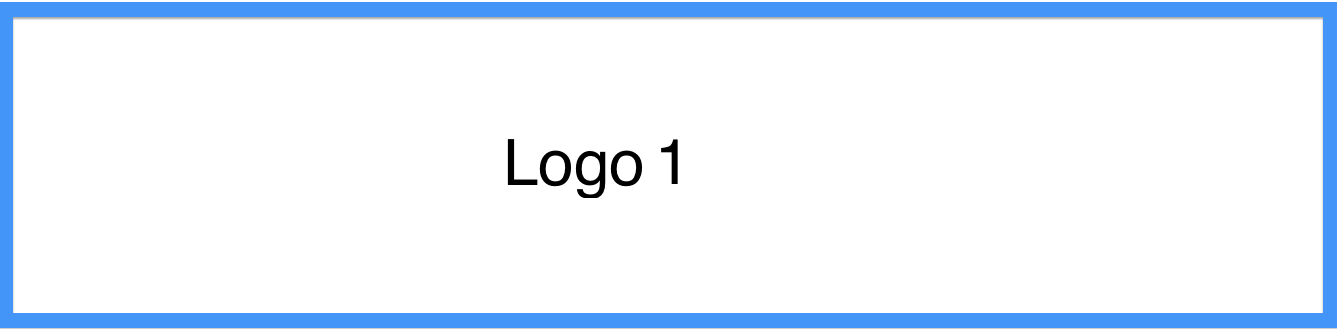
\includegraphics[width=0.3\textwidth,angle=0]{abb/logo1}
 \caption[Abbildung im Anhang]{Abbildung im Anhang}
\label{fig:Abbildung im Anhang}
\end{figure}

Lorem ipsum dolor sit amet, consetetur sadipscing elitr, sed diam nonumy eirmod tempor invidunt ut labore et dolore magna aliquyam erat, sed diam voluptua. At vero eos et accusam et justo duo dolores et ea rebum. Stet clita kasd gubergren, no sea takimata sanctus est Lorem ipsum dolor sit amet. Lorem ipsum dolor sit amet, consetetur sadipscing elitr, sed diam nonumy eirmod tempor invidunt ut labore et dolore magna aliquyam erat, sed diam voluptua. At vero eos et accusam et justo duo dolores et ea rebum. Stet clita kasd gubergren, no sea takimata sanctus est Lorem ipsum dolor sit amet.


% Eidesstattliche Erklärung
\newpage
\addcontentsline{toc}{section}{Eidesstattliche Erklärung}
\section*{Eidesstattliche Erklärung}
\thispagestyle{empty}

\begin{verbatim}

\end{verbatim}

\begin{LARGE}Eidesstattliche Erklärung zur <-Arbeit>\end{LARGE}
\begin{verbatim}


\end{verbatim}
Ich versichere, die von mir vorgelegte Arbeit selbstständig verfasst zu haben. Alle Stellen, die wörtlich oder sinngemäß aus veröffentlichten oder nicht veröffentlichten Arbeiten anderer entnommen sind, habe ich als entnommen kenntlich gemacht. Sämtliche Quellen und Hilfsmittel, die ich für die Arbeit benutzt habe, sind angegeben. Die Arbeit hat mit gleichem Inhalt bzw. in wesentlichen Teilen noch keiner anderen Prüfungsbehörde vorgelegen.



\begin{displaymath}
% use packages: array
\begin{array}{ll}
Unterschrift:~~~~~~~~~~~~~~~~~~~~~~~~~~~~~~~~~~~~~~~~~~
& Ort, Datum:~~~~~~~~~~~~~~~~~~~~~~~~~~~~~~~~~~~~~~~~~~
\end{array}
\end{displaymath}



\end{document}
